\documentclass{beamer}
\usefonttheme[onlymath]{serif}
\usepackage[T1]{fontenc}
\usepackage[utf8]{inputenc}
\usepackage[english]{babel}
\usepackage{amsmath}
\usepackage{amssymb}
\usepackage{amsthm}
\usepackage{gensymb}
\usepackage{parskip}
\usepackage{mathtools}
\usepackage{listings}
\usepackage{hyperref}
\usepackage{graphicx}
\usepackage{color}
\usepackage{enumerate}
\usepackage{tikz}
\usetikzlibrary{calc}
\usetikzlibrary{positioning}
\usetikzlibrary{angles}
\usetikzlibrary{shapes}
\usetikzlibrary{arrows}
\usepackage{verbatim}
\usepackage{multicol}
\usepackage{array}
\usepackage{minted}
\parskip 0pt


\DeclareMathOperator{\lcm}{lcm}
\newcommand\floor[1]{\left\lfloor#1\right\rfloor}
\newcommand\ceil[1]{\left\lceil#1\right\rceil}
\newcommand\abs[1]{\left|#1\right|}
\newcommand\p[1]{\left(#1\right)}
\newcommand\sqp[1]{\left[#1\right]}
\newcommand\cp[1]{\left\{#1\right\}}
\newcommand\norm[1]{\left\lVert#1\right\rVert}
\renewcommand\Im{\operatorname{Im}}
\renewcommand\Re{\operatorname{Re}}

\usetheme{metropolis}
\definecolor{dark yellow}{rgb} {0.6,0.6,0.0}
\definecolor{dark green}{rgb} {0.0,0.6,0.0}

\graphicspath{{myndir/}}

\title{Reduce and conquer}
\author{Atli FF}
\institute{\href{http://ru.is/td}{School of Computer Science} \\[2pt] \href{http://ru.is}{Reykjavík University}}
\titlegraphic{\hfill\includegraphics[height=0.6cm]{kattis}}

\begin{document}
\maketitle

\begin{frame}[plain]{Divide and conquer}
    \begin{itemize}
        \item Given an instance of the problem, the basic idea is to
        \begin{enumerate}
            \item split the problem into one or more smaller subproblems
            \item solve each of these subproblems recursively
            \item combine the solutions to the subproblems into a solution of the given problem
        \end{enumerate}

        \vspace{5pt}

        \item Some standard divide and conquer algorithms:
        \begin{itemize}
            \item Quicksort / Mergesort
            \item Karatsuba algorithm
            \item Strassen algorithm
            \item Many algorithms from computational geometry
                \begin{itemize}
                    \item Convex hull
                    \item Closest pair of points
                \end{itemize}
        \end{itemize}
    \end{itemize}
\end{frame}

\begin{frame}[plain,fragile]{Divide and conquer: Time complexity}
    \begin{minted}[fontsize=\scriptsize]{cpp}
void solve(int n) {
    if (n == 0)
        return;

    solve(n/2);
    solve(n/2);

    for (int i = 0; i < n; i++) {
        // some constant time operations
    }
}
    \end{minted}

    \begin{itemize}
        \item What is the time complexity of this divide and conquer algorithm?
        \item Usually helps to model the time complexity as a recurrence relation:
            \begin{itemize}
                \item $T(n) = 2T(n/2) + n$
            \end{itemize}
    \end{itemize}
\end{frame}

\begin{frame}[plain,fragile]{Divide and conquer: Time complexity}
    \begin{itemize}
        \item But how do we solve such recurrences?
        \item Usually simplest to use the Master theorem when applicable
            \begin{itemize}
                \item It gives a solution to a recurrence of the form $T(n) = aT(n/b) + f(n)$ in asymptotic terms
                \item All of the divide and conquer algorithms mentioned so far have a recurrence of this form
            \end{itemize}
        \vspace{10pt}
        \item The Master theorem tells us that $T(n) = 2T(n/2) + n$ has asymptotic time complexity $O(n \log n)$
        \vspace{10pt}
        \item You don't need to know the Master theorem for this course, but still recommended as it's very useful
    \end{itemize}
\end{frame}

\begin{frame}[plain]{Reduce and conquer}
    \begin{itemize}
        \item Sometimes we're not actually dividing the problem into many subproblems, but only into one smaller subproblem
        \item Usually called reduce and conquer
        \item The most common example of this is binary search
        \item We will look at reduce and conquer this week, and more general divide and conquer algorithms next week
    \end{itemize}
\end{frame}

\begin{frame}[plain]{Binary search}
    \begin{itemize}
        \item We have a \textbf{sorted} array of elements, and we want to check if it contains a particular element $x$
        \vspace{5pt}
        \item Algorithm:
        \begin{enumerate}
            \item Base case: the array is empty, return false
            \item Compare $x$ to the element in the middle of the array
            \item If it's equal, then we found $x$ and we return true
            \item If it's less, then $x$ must be in the left half of the array
            \begin{enumerate}
                \item Binary search the element (recursively) in the left half
            \end{enumerate}
            \item If it's greater, then $x$ must be in the right half of the array
            \begin{enumerate}
                \item Binary search the element (recursively) in the right half
            \end{enumerate}
        \end{enumerate}
    \end{itemize}
\end{frame}

\begin{frame}[plain,fragile]{Binary search}
    \begin{minted}[fontsize=\scriptsize]{cpp}
bool binary_search(const vector<int> &arr, int lo, int hi, int x) {
    if (lo > hi) {
        return false;
    }

    int m = (lo + hi) / 2;
    if (arr[m] == x) {
        return true;
    } else if (x < arr[m]) {
        return binary_search(arr, lo, m - 1, x);
    } else if (x > arr[m]) {
        return binary_search(arr, m + 1, hi, x);
    }
}

binary_search(arr, 0, arr.size() - 1, x);
    \end{minted}

    \begin{itemize}
        \item $T(n) = T(n/2) + 1$
        \item $O(\log n)$
    \end{itemize}
\end{frame}

\begin{frame}[plain,fragile]{Binary search - iterative}
    \begin{minted}[fontsize=\scriptsize]{cpp}
bool binary_search(const vector<int> &arr, int x) {
    int lo = 0,
        hi = arr.size() - 1;

    while (lo <= hi) {
        int m = (lo + hi) / 2;
        if (arr[m] == x) {
            return true;
        } else if (x < arr[m]) {
            hi = m - 1;
        } else if (x > arr[m]) {
            lo = m + 1;
        }
    }

    return false;
}
    \end{minted}
\end{frame}

\begin{frame}[plain]{Binary search over integers}
    \begin{itemize}
        \item This might be the most well known application of binary search, but it's far from being the only application
        \item More generally, we have a predicate $p : \{0,\ldots,n-1\} \rightarrow \{T, F\}$ which has the property that if $p(i) = T$, then $p(j) = T$ for all $j > i$
        \item Our goal is to find the smallest index $j$ such that $p(j) = T$ as quickly as possible
    \end{itemize}

    \begin{center}
        \begin{tabular}{ccccccccccccccccccc}
            $i$ & $0$ & $1$ & $\cdots$ & $j-1$ & \color{blue}{$j$} & $j+1$ & $\cdots$ & $n-2$ & $n-1$ \\
            \hline
            $p(i)$ & $F$ & $F$ & $\cdots$ & $F$ & \color{blue}{$T$} & $T$ & $\cdots$ & $T$ & $T$ \\
        \end{tabular}
    \end{center}

    \begin{itemize}
        \item We can do this in $O(\log(n) \times f)$ time, where $f$ is the cost of evaluating the predicate $p$, in the same way as when we were binary searching an array
    \end{itemize}
\end{frame}

\begin{frame}[plain,fragile]{Binary search over integers}
    \begin{minted}[fontsize=\footnotesize]{cpp}
int lo = 0,
    hi = n - 1;

while (lo < hi) {
    int m = (lo + hi) / 2;

    if (p(m)) {
        hi = m;
    } else {
        lo = m + 1;
    }
}

if (lo == hi && p(lo)) {
    printf("lowest index is %d\n", lo);
} else {
    printf("no such index\n");
}
    \end{minted}
\end{frame}

\begin{frame}[plain,fragile]{Binary search over reals}
    \begin{itemize}
        \item An even more general version of binary search is over the real numbers
        \item We have a predicate $p : [lo,hi] \rightarrow \{T, F\}$ which has the property that if $p(i) = T$, then $p(j) = T$ for all $j > i$
        \item Our goal is to find the smallest real number $j$ such that $p(j) = T$ as quickly as possible

        \vspace{5pt}
        \item Since we're working with real numbers (hypothetically), our $[lo,hi]$ can be halved infinitely many times without ever becoming a single real number
        \item Instead it will suffice to find a real number $j'$ that is very close to the correct answer $j$, say not further than $EPS = 2^{-30}$ away, we can do this in $O(\log(\frac{hi - lo}{EPS}))$ time in a similar way as when we were binary searching an array
    \end{itemize}
\end{frame}

\begin{frame}[plain]{Example}
	\begin{center}
		\begin{tikzpicture}
			[domain = -0.2:4.2]
			\draw[->] (-0.2,0) -- (4.2,0);
			\draw[->] (0,-0.2) -- (0,4.2);
			\draw[color=red] plot[id=c] function{2} node[right] {$y$};
			\draw[color=blue] plot[id=poly3] function{0.9 + 1.08333*x - 0.75*x**2 + 0.166667*x**3} node[right] {$f(x)$};



			\node<all:1-2>[below] at (0.7,-0.125) {$a$};
			\draw<all:1-2> (0.7,0.125) -- (0.7,-0.125);
			\draw<all:1-2>[dashed, gray] (0.7,0.125) -- (0.7, 4.2);
			\node<all:1-6>[below] at (3.7,-0.125) {$b$};
			\draw<all:1-6>(3.7,0.125) -- (3.7,-0.125);
			\draw<all:1-6>[dashed, gray] (3.7,0.125) -- (3.7,4.2);

			\node<all:2>[below] at (2.2,-0.125) {$m$};
			\draw<all:2-4> (2.2,0.125) -- (2.2,-0.125);
			\draw<all:2-4>[dashed, gray] (2.2,0.125) -- (2.2,4.2);

			\node<all:3-4>[below] at (2.2,-0.125) {$a$};

			\node<all:4>[below] at (2.95,-0.125) {$m$};
			\draw<all:4-> (2.95,0.125) -- (2.95,-0.125);
			\draw<all:4->[dashed, gray] (2.95,0.125) -- (2.95,4.2);

			\node<all:5->[below] at (2.95,-0.125) {$a$};

			\node<all:6>[below] at (3.325,-0.125) {$m$};
			\draw<all:6-> (3.325,0.125) -- (3.325,-0.125);
			\draw<all:6->[dashed, gray] (3.325,0.125) -- (3.325,4.2);

			\node<all:7->[below] at (3.325,-0.125) {$b$};
        \end{tikzpicture}
    \end{center}
\end{frame}

\begin{frame}[plain,fragile]{Binary search over reals}
    \begin{minted}{cpp}
double EPS = 1e-10,
       lo = -1000.0,
       hi = 1000.0;

while (hi - lo > EPS) {
    double mid = (lo + hi) / 2.0;

    if (p(mid)) {
        hi = mid;
    } else {
        lo = mid;
    }
}

printf("%0.10lf\n", lo);
    \end{minted}
\end{frame}

\begin{frame}[plain,fragile]{Binary search over reals}
    \begin{itemize}
        \item This has many cool numerical applications
        \vspace{5pt}
        \item Find the square root of $x$
    \end{itemize}
    \begin{minted}{cpp}
bool p(double j) {
    return j*j >= x;
}
    \end{minted}
    \begin{itemize}
        \item Find the root of an increasing function $f(x)$
    \end{itemize}
    \begin{minted}{cpp}
bool p(double x) {
    return f(x) >= 0.0;
}
    \end{minted}

    \begin{itemize}
        \item This is also referred to as the Bisection method
    \end{itemize}
\end{frame}

\begin{frame}[plain]{Binary search the answer}
    \begin{itemize}
        \item It may be hard to find the optimal solution directly, as we saw in the example problem
        \item On the other hand, it may be easy to check if some $x$ is a solution or not
        \vspace{5pt}
        \item A method of using binary search to find the minimum or maximum solution to a problem
        \item Only applicable when the problem has the binary search property: if $i$ is a solution, then so are all $j > i$
        \vspace{5pt}
        \item $p(i)$ checks whether $i$ is a solution, then we simply apply binary search on $p$ to get the minimum or maximum solution
    \end{itemize}
\end{frame}

\begin{frame}[plain]{Ternary search}
    \begin{itemize}
        \item Another useful and similar algorithm is ternary search
        \item This time we have a convex function $f$ ($f'' \geq 0$), so it might decrease at first and then increase
        \item This function will have a unique minimum value that we might want to find, perhaps to minimize some cost function
        \item This can be done in a similar fashion to binary search
    \end{itemize}
\end{frame}

\begin{frame}[plain]{Ternary search}
	\begin{itemize}
        \item We choose points $m_1, m_2$ in our interval $[a, b]$ so $[a, m_1]$, $[m_1, m_2]$ and $[m_2, b]$ are equally large.
        \item We then consider $f(m_1), f(m_2)$.
        \item If $f(m_1) < f(m_2)$ the minimum can not be in $[m_2, b]$ so we can discard it.
        \item If $f(m_2) < f(m_1)$ the minimum can not be in $[a, m_1]$ so we can discard it.
        \item If $f(m_1) = f(m_2)$ the minimum must be in $[m_1, m_2]$.
        \item This can be shown to be true using analysis, since convex functions take their maxima on the endpoints of intervals.
    \end{itemize}
\end{frame}

\begin{frame}{Example}
	\begin{center}
		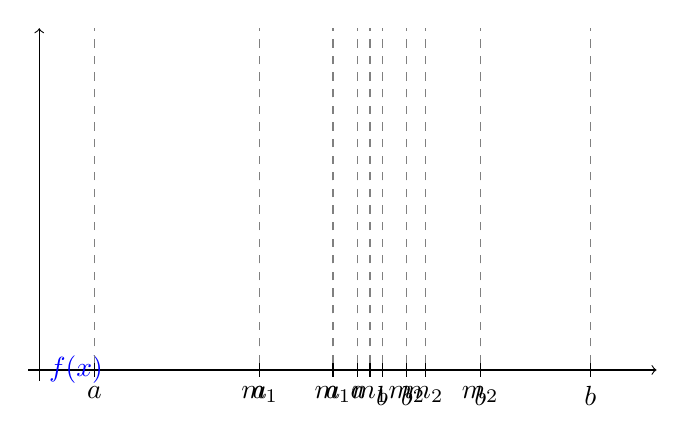
\begin{tikzpicture}[scale = 0.7, domain=-0.2:11.2]
			\draw[->] (-0.2,0) -- (11.2,0);
			\draw[->] (0,-0.2) -- (0,6.2);
			\draw[color = blue] plot[id=poly2] function{5 - 1.2*x + 0.1*x**2} node[right] {$f(x)$};

			\node<all:1-2>[below] at (1,-0.125) {$a$};
			\draw<all:1-2> (1,0.125) -- (1,-0.125);
			\draw<all:1-2>[dashed, gray] (1,0.125) -- (1, 6.2);

			\node<all:1-4>[below] at (10,-0.125) {$b$};
			\draw<all:1-4>(10,0.125) -- (10,-0.125);
			\draw<all:1-4>[dashed, gray] (10,0.125) -- (10,6.2);

			\node<all:2>[below] at (4,-0.125) {$m_1$};
			\draw<all:2>(4,0.125) -- (4,-0.125);
			\draw<all:2>[dashed, gray] (4,0.125) -- (4,6.2);

			\node<all:2>[below] at (7,-0.125) {$m_2$};
			\draw<all:2>(7,0.125) -- (7,-0.125);
			\draw<all:2>[dashed, gray] (7,0.125) -- (7,6.2);

			\node<all:3-6>[below] at (4,-0.125) {$a$};
			\draw<all:3-6> (4,0.125) -- (4,-0.125);
			\draw<all:3-6>[dashed, gray] (4,0.125) -- (4, 6.2);

			\node<all:4>[below] at (6,-0.125) {$m_1$};
			\draw<all:4>(6,0.125) -- (6,-0.125);
			\draw<all:4>[dashed, gray] (6,0.125) -- (6,6.2);

			\node<all:4>[below] at (8,-0.125) {$m_2$};
			\draw<all:4>(8,0.125) -- (8,-0.125);
			\draw<all:4>[dashed, gray] (8,0.125) -- (8,6.2);

			\node<all:5-6>[below] at (8,-0.125) {$b$};
			\draw<all:5-6>(8,0.125) -- (8,-0.125);
			\draw<all:5-6>[dashed, gray] (8,0.125) -- (8,6.2);

			\node<all:6>[below] at (5.33,-0.125) {$m_1$};
			\draw<all:6>(5.33,0.125) -- (5.33,-0.125);
			\draw<all:6>[dashed, gray] (5.33,0.125) -- (5.33,6.2);

			\node<all:6>[below] at (6.67,-0.125) {$m_2$};
			\draw<all:6>(6.67,0.125) -- (6.67,-0.125);
			\draw<all:6>[dashed, gray] (6.67,0.125) -- (6.67,6.2);

			\node<all:7-8>[below] at (5.33,-0.125) {$a$};
			\draw<all:7-8>(5.33,0.125) -- (5.33,-0.125);
			\draw<all:7-8>[dashed, gray] (5.33,0.125) -- (5.33,6.2);

			\node<all:7-8>[below] at (6.67,-0.125) {$b$};
			\draw<all:7-8>(6.67,0.125) -- (6.67,-0.125);
			\draw<all:7-8>[dashed, gray] (6.67,0.125) -- (6.67,6.2);

			\draw<all:8>(5.78,0.125) -- (5.78,-0.125);
			\draw<all:8>[dashed, gray] (5.78,0.125) -- (5.78,6.2);

			\draw<all:8>(6.22,0.125) -- (6.22,-0.125);
			\draw<all:8>[dashed, gray] (6.22,0.125) -- (6.22,6.2);

			\node<all:9>[below] at (5.78,-0.125) {$a$};
			\draw<all:9>(5.78,0.125) -- (5.78,-0.125);
			\draw<all:9>[dashed, gray] (5.78,0.125) -- (5.78,6.2);

			\node<all:9>[below] at (6.22,-0.125) {$b$};
			\draw<all:9>(6.22,0.125) -- (6.22,-0.125);
			\draw<all:9>[dashed, gray] (6.22,0.125) -- (6.22,6.2);
		\end{tikzpicture}
    \end{center}
\end{frame}


\end{document}
